% !TEX encoding = UTF-8 Unicode
\documentclass[a4paper]{article}

\usepackage{color}
\usepackage{xcolor}
\usepackage{url}
\usepackage[T2A]{fontenc} % enable Cyrillic fonts
\usepackage[utf8]{inputenc} % make weird characters work
\usepackage{graphicx}
\usepackage{listings}
\usepackage[english,serbian]{babel}
%\usepackage[english,serbianc]{babel} %ukljuciti babel sa ovim opcijama, umesto gornjim, ukoliko se koristi cirilica

\usepackage[unicode]{hyperref}
\hypersetup{colorlinks,citecolor=green,filecolor=green,linkcolor=blue,urlcolor=blue}

%\newtheorem{primer}{Пример}[section] %ćirilični primer
\newtheorem{primer}{Primer}[section]

\definecolor{mygreen}{rgb}{0,0.6,0}
\definecolor{mygray}{rgb}{0.5,0.5,0.5}
\definecolor{mymauve}{rgb}{0.58,0,0.82}
\definecolor{commentgreen}{RGB}{2,112,10}
\definecolor{eminence}{RGB}{108,48,130}
\definecolor{weborange}{RGB}{255,165,0}
\definecolor{frenchplum}{RGB}{129,20,83}
\definecolor{pink}{rgb}{0.858,0.188,0.478}

\lstdefinelanguage{Elixir}{
    morekeywords={case,catch,def,do,else,false,%
        use,alias,receive,timeout,defmacro,defp,%
        for,if,import,defmodule,defprotocol,%
        nil,defmacrop,defoverridable,defimpl,%
        super,fn,raise,true,try,end,with,%
        unless},
    otherkeywords={<-,->, |>, \%\{, \}, \{, \, (, )},
    keywords=[2]{IO},
    keywords=[3]{iex},
    sensitive=true,
    morecomment=[l]{\#},
    morecomment=[n]{/*}{*/},
    morecomment=[s][\color{purple}]{:}{\ },
    morestring=[s][\color{orange}]"",
    commentstyle=\color{commentgreen},
    keywordstyle=\color{eminence},
    keywordstyle=[2]\color{pink},
    keywordstyle=[3]\color{mygreen},
    stringstyle=\color{red},
	basicstyle=\ttfamily,
	breaklines,
	showstringspaces=false,
	frame=tb
}

\lstset{ 
  backgroundcolor=\color{white},   % choose the background color; you must add \usepackage{color} or \usepackage{xcolor}; should come as last argument
  basicstyle=\scriptsize\ttfamily,        % the size of the fonts that are used for the code
  breakatwhitespace=false,         % sets if automatic breaks should only happen at whitespace
  breaklines=true,                 % sets automatic line breaking
  captionpos=b,                    % sets the caption-position to bottom
  commentstyle=\color{mygreen},    % comment style
  deletekeywords={...},            % if you want to delete keywords from the given language
  escapeinside={\%*}{*)},          % if you want to add LaTeX within your code
  extendedchars=true,              % lets you use non-ASCII characters; for 8-bits encodings only, does not work with UTF-8
  firstnumber=1000,                % start line enumeration with line 1000
  frame=single,	                   % adds a frame around the code
  keepspaces=true,                 % keeps spaces in text, useful for keeping indentation of code (possibly needs columns=flexible)
  keywordstyle=\color{blue},       % keyword style
  language=Elixir,                 % the language of the code
  morekeywords={*,...},            % if you want to add more keywords to the set
  numbers=left,                    % where to put the line-numbers; possible values are (none, left, right)
  numbersep=5pt,                   % how far the line-numbers are from the code
  numberstyle=\tiny\color{mygray}, % the style that is used for the line-numbers
  rulecolor=\color{black},         % if not set, the frame-color may be changed on line-breaks within not-black text (e.g. comments (green here))
  showspaces=false,                % show spaces everywhere adding particular underscores; it overrides 'showstringspaces'
  showstringspaces=false,          % underline spaces within strings only
  showtabs=false,                  % show tabs within strings adding particular underscores
  stepnumber=2,                    % the step between two line-numbers. If it's 1, each line will be numbered
  stringstyle=\color{mymauve},     % string literal style
  tabsize=2,	                   % sets default tabsize to 2 spaces
  title=\lstname                   % show the filename of files included with \lstinputlisting; also try caption instead of title
}

\begin{document}

\title{Naslov seminarskog rada\\ \small{Seminarski rad u okviru kursa\\Metodologija stručnog i naučnog rada\\ Matematički fakultet}}

\author{Prvi autor, drugi autor, treći autor, četvrti autor\\ kontakt email prvog, drugog, trećeg, četvrtog autora}

%\date{9.~april 2015.}

\maketitle

\abstract{
U ovom tekstu je ukratko prikazana osnovna forma seminarskog rada. Obratite pažnju da je pored ove .pdf datoteke, u prilogu i odgovarajuća .tex datoteka, kao i .bib datoteka korišćena za generisanje literature. Na prvoj strani seminarskog rada su naslov, apstrakt i sadržaj, i to sve mora da stane na prvu stranu! Kako bi Vaš seminarski zadovoljio standarde i očekivanja, koristite uputstva i materijale sa predavanja na temu pisanja seminarskih radova. Ovo je samo šablon koji se odnosi na fizički izgled seminarskog rada (šablon koji \emph{morate} da koristite!) kao i par tehničkih pomoćnih uputstava. Pročitajte tekst pažljivo jer on sadrži i važne informacije vezane za zahteve obima i karakteristika seminarskog rada.}

\tableofcontents

\newpage

\section{Uvod}
\label{sec:uvod}

Elixir(Eliksir) je programski jezik koji se prvi put pojavljuje u javnosti 2012. godine kao projekat kompanije Plataformatec. Ovaj funkcionalni, dinamičan programski jezik*(footnote: Diskusija o specificnoj paradigmi u daljem tekstu) se pokreće na Erlang vituelnoj mašini pa samim tim i deli pogodna svojstva kao što su konkurentnost i tolerisanje grešaka, koje dolaze sa ovim okruženjem. Njegov tvorac, Jose Valim, navodi da je motivacija za pravljenje ovog jezika upravo bila ljubav prema ovoj virtualnoj mašini i ekosistemu, ali i njeni nedostaci. Iz tačke gledišta olakšavanja svakodnevnog razvoja sofvera, koncepti poput metaprogramiranje - tehnika kojom programi imaju mogućnost da druge programe posmatraju kao svoje podatke i na taj način čitaju pa čak i modifikuju njihov, a samim tim i svoj kod u vreme izvršavanja, zatim polimorfizam (pretp. da čitaoc zna, pitati prof.) i makroi kao i podrška za alate, bili su neke od nepostojećih karakteristika ovog sistema koje bi Elixir trebalo da nadomesti. Cilj ovog rada je da čitaoca bliže upozna sa osobinama, funkcionalnostima i specifičnostima ovog jezika kao i da kroz uporedni prikaz sa jezicima koji dele slične kocepte ili imaju istu upotrebu u određenim domenima, prikaže mane i prednosti Elixira.
% Kada budete predavali seminarski rad, imenujete datoteke tako da sadrže redni broj teme, temu seminarskog rada, kao i prezimena članova grupe. Precizna uputstva na temu imenovnja će biti data na formi za predaju seminarskog rada. Predaja seminarskih radova biće isključivo preko veb forme, a NE slanjem mejla. Link na formu će biti dat u okviru obaveštenja na strani kursa. Vodite računa da prilikom predavanja seminarskog rada predate samo one fajlove koji su neophodni za ponovno generisanje pdf datoteke. To znači da pomoćne fajlove, kao što su .log, .out, .blg, .toc, .aux i slično, \textbf{ne treba predavati}.

\section{Istorijat}
\label{sec:istorijat}

Tokom 1980ih, telekomunikaciona kompanija Ericsson ispitivala je problem konkurentnosti, i nakon izvršenih testiranja odlučila je da razvije svoj jezik koji bi bio zasnovan na ovoj funkcionalnosti: Erlang. U to vreme brojnost jezika nije bila velika, kao danas. Programski jezik C je bio najzastupljeniji, ali uprkos njegovoj prilagodljivosti, tri programera Joe Armstrong, Mike Williams i Robert Virding, koji su bili zaposleni u Ericsson-u, su shvatili da mogu biti produktivniji ukoliko koriste programski jezik višeg nivoa. Nakon eksperimenata sa postojećim jezicima, odlučili su se da ni jedan ne zadovoljava njihove potrebe u dovoljnoj meri, pa su tokom 1987. započeli pisanje Erlanga i predstavili ga tri godine kasnije.

Jezik je najviše korišćen od strane telekomunikacionih kompanija, a glavni fokus je bila distribucija, tolerantnost na otkaze u sistemu, i hot-swappinga koda (mogućnost izmene koda programa bez potrebe prekida izvršavanja). U 1998. Ericsson se odlučuje da kod programskoj jezika Erlang učini dostupan svima i proglašava ga otvorenim (open source). Od tada je jezik korišćen u veoma specifičnim projektima, kao što je dobro poznati broker za poruke RabbitMQ, XMPP server “ejabberd”, i Apache CouchDB, koji je jedna od najpoznatijih distribuiranih baza podataka. Neke kompanije koriste Erlang za telekomunikacione proizvode, a primer su WhatsApp i Riot Games - kompanija koja je napravila igru League of Legends.

Tokom 2010., Jose Valim, u to vreme zaposlen na poziciji programera u kompaniji Plataformatec, radio je na poboljšanju performansi Ruby on Rails framework-a na višejezgarnim sistemima i bio je sve više frustriran ovim poslom. Shvatio je da Ruby nije bio dovoljno dobro dizajniran da reši problem konkurentnosti, pa je započeo istraživanje drugih tehnologija koje bi bile prihvatljivije. Tako je otkrio Erlang, i upravo ga je interesovanje prema Erlangovoj virtuelnoj mašini podstaklo da započne pisanje Elixira. Uticaj projekta na kome je do tada radio odrazio se na to da Elixir ima sintaksu koja je nalik na Ruby-jevu. Ovaj jezik se pokazao veoma dobro pri upravljanju milionima simultanih konekcija: u 2015. Phoenix - zabeleženo upravljanje 2 miliona WebSocket konekcija, dok je u 2017. za skalirani Elixir zabeležena obrada 5 miliona istovremenih korisnika. (Q: Mozda bismo mogli neki grafik ili sliku o ovome) Elixir se danas koristi u velikim kompanijama, kao što su Pinterest, Moz, a upotrebu nalazi čak i u bankarskim sistemima. (q: pitati jel medium relevantan)( ref: https://medium.com/margobank/why-elixir-546427542c)

\section{BEAM - Erlang virtualna masina}

Kako je Elixir zapravo nastao proširivanjem funkcionalnosti BEAM-a (Erlangove virtualne mašine), sa ciljem da se zadrži kompatibilnost sa Erlang ekosistemom, važno je opisati osnovne koncepte funkcionisanja Erlang virtualne mašine na kojoj se  kompajlirani Elixir kod izvršava.

Originalno BEAM je bila skraćenica za Bogdan's Erlang Abstract Machine, po Bogumil "Bogdan" Hausman koji je napisao originalnu verziju virtualne mašine, ali ime se takođe moze tumačiti kao Björn's Erlang Abstract Machine, po Björn Gustavsson, koji piše i održava trenutnu verziju.

BEAM predstavlja jezgro Erlang Open Telecom Platform (Erlang/OTP), platforme koja se sastoji od Erlang Run-Time System(ERTS) i  kolekcije unapred kompajliranih middleware, biblioteka i alata pisanih u Erlangu.

Erlang Run-Time System (ERTS) predstavlja modul zadu\v{z}en za kompilaciju Erlang i Elixir izvornog koda u bytecode koji se onda izvršava u okviru BEAM-a.

U okviru BEAM-a, sav kod se izvršava u sitnim konkurentnim procesima, pri čemu procesi nisu procesi operativnog sistema, vec Erlang procesi, što je moguće upravo zbog izvršavanja u okviru BEAM virtualne mašine. Svaki od procesa je memorijski nezavistan i sva međuprocesna komunikacije se odvija razmenjivanjem poruka, čime se obezbeđuje koncept konkurentnosti slanjem poruka \textit{(eng. message passing concurrency)}. 

Prevo]enjem Elixir izvornog fajla generise se .beam fajl koji sadrzi bytecode koji se može izvršavati u okviru BEAM-a.

\section{Osobine jezika}
\label{sec:osobine}
U ovom poglavlju(q: da li su ovo naslovi poglavja) će biti opisane osobine Elixira, osnove njegove sintakse, semantike, kao i podrška za koncepte koji su odlike funkcionalnih i konkurentnih jezika. (q: mesanje vremena) 

Pre nego što započnemo priču o tipovima, bitno je osvrnuti se na koncepte \textit{Patter matching}-a i \textit{Imutabilnosti} promenjivih kao i reći nešto o \textbf{Kernelu}. To je podrazumevano okruženje koje se koristi u Elixiru. Ono sadrži primitive jezika kao što su: \textit{aritmetičke operacije}, rukovanje \textit{procesima} i \textit{tipovima}, \textit{makroe} za definisanje novih funkcionalnosti (\textit{funkcija, modula...}), provere \textit{guard-ova} - predefinisanog skupa funkcija i makroa koji proširuju mogućnost \textit{pattern matching}-a itd. Sve ove funkcionalnosti se mogu pozivati bez prefiksa \textit{Kernel} jer su podrazumevano importovane po pokretanju interpretera (ovo važi i ukoliko se program kompajlira). Ukoliko pak korisnik ne želi da uključi pojedine funkcije/makroe može to uraditi korisćenjem \textbf{:except} opcije \textit{import} funkcije. (t: primer)

\subsection{Pattern matching}
\label{sec:pattern}
Definicija \textit{pattern matching}-a bi glasila ovako: proveravanje da li se u data sekvenci tokena može prepoznati neki šablon. Na praktičnom primeru operatora = ovaj koncept će biti jasniji. 
U većini programskih jezika, operator = je operator dodele, koji levoj strani dodeljuje vrednost izraza na desnoj. U Elixiru ovaj operator, koji se naziva operator \textit{uparivanja} (eng:\textit{matching}) ima drugačiju funkciju koja više podseća na \textit{assertion}. On se uspešno izvršava ako pronađe načina da izjadnači levu stanu (svoj prvi operand) \textit{sa} desnom (drugi perand).
\begin{primer}
U narednom parčetu koda \textit{a} je promenljiva koja uspeva da se izjednači sa vrednoću 1, tako sto biva postavljena na tu vrednost. U drugoj naredbi izvršavanje operacije ponovo uspeva jer je vrednost leve strane 1 dok promenljiva sa desne strane već ima vrednost 1 zbog prethodne operacije. Neuspeh sledeće naredbe može izgledati neintuitivno, ali kada se bolje pogleda objašnjenje ove operacija trebalo bi da bude jasno. Naime, Elixir pokušava da izjednači levu stranu, koja je broj 2, koji može imati samo tu vrednosti, sa promenjivom \textit{a} koja ima vrednost 1. Ključna stvar za razumeti je da Elixir ne pokušava da izjednači levu \textit{i} desnu stranu, već levu \textit{sa} desnom.
\end{primer}
\begin{lstlisting}[caption={Primer jednostavnog pattern matchinga},frame=single, label=simple]
iex> a = 1
# 1
iex> 1 = a
# 2
iex> 2 = a
#(MatchError) no match of right hand side value: 1
\end{lstlisting}
\subsection{Imutabilnost}
\label{sec:tipovi}
Imajući na umu funkcionalnu paradigmu Elixira, imutabilnost podataka je osobina koja je neizostavna. Naime, jednom kreirani podaci ne mogu mogu biti promenjeni. Bez ulaženja u dublje analize rasprava o tome da li je mutabilnost podataka dobra ili loša, činjenica je da postojanje stanja i funkcija, koje to stanje mogu menjati u izrazima sa bočnim efektima, otežava razumevanje i još bitnije, utvrđivanje korektnosti funkcionisanja sistema. Pogotovo u slučaju višenitnih, konkurentnih ili distribuiranih programa, kakvi se najčešće pišu korićenjem Elixir programskog jezika. 
\subsection{Ugrađeni tipovi}
\label{sec:tipovi}
Elixir implementira desetine tipova. Od njih je važno istaći ugradjene - primitivne tipova, preko kojih su realizovane implementacije ostalih:
\begin{itemize}
  \item Atomi (\textit{Atom})
  \item Celi brojevi (\textit{Integer})
  \item Brojevi u pokretnom zarezu(\textit{Float})
  \item Procesi (\textit{Process})
  \item Portovi (\textit{Port})
  \item Uređene torke (\textit{Tuple})
  \item Liste (\textit{List})
  \item Mape (\textit{Map})
  \item Funkcije (\textit{Function})
  \item Niske bitova 
  \item Reference
\end{itemize}

U zagradama nakon tipa, osim u poslednja dva koji nemaju odgovarajuće module, navena su imena modula koji sadrže funckije koje se koriste za operacije nad tim tipom. Imena ovih modula ne treba mešati sa primitivnim tipovima navedenim gore, iako oni sami jesu tip. Oni se mogu zamisliti kao neka vrsta omotača oko primitivnog tipa koji obezbedjuje bogatije funkcionalnosti nad njime. 
\begin{primer}
Literal [...] može biti iskorišćen da se napravi lista (primitiva), nad njom je moguće iskoristiti operator | koji bi je dekomponovao na glavu i rep ili od nje napravio novu listu (detalji u predstojećim poglavljima). U modulu \textit{List} imamo funkciju \textit{last} koja kada se primeni na listu, kao rezultat vraća njen poslednji element.
\end{primer}

Može biti čudno što se na ovoj listi nisu našle niske ili strukture, ali one su deo složenih tipova podržanih od strane Elixira. Takodje, postoji debata o tome da li su regularni izrazi i opsezi (\textit{Ranges}) tipovi za sebe i u nekoj literaturi se posmatraju ovako iako su tehnički strukture. (ref: Programming Elixir 1.3)

\subsubsection{Atomi, celi i brojevi u pokretno zarezu i opsezi}
\label{sec:ime}
\textit{Atomi} su konstante koje predstavljaju ime. Počinju dvotačkom i njihovo je ime im je i vrednost, šsto znači da će dva atoma sa istim imenom pri poređenju uvek biti isti bez obzira na to da li su kreirani od strane različitih aplikacija.

\textit{Celi brojevi} su slični kao i u većini drugih jezika i mogu se obeležavati korišćenjem dekadne (1234), heksadekadne (0xcafe), oktalne (0o1234) i binarne (0b1010) notacije. Karakter \_ se može koristiti za odvajanje blokova cifara. Bitna stvar je da ne postoji fiksna veličina za čuvanje celih brojeva u memoriji, već se interna reprezentacija raste kako bi obezbedila da broj bude smešten.

\textit{Brojevi u pokretnom zarezu} se u memoriji zapisuju po standardu IEEE 754 (q: ref:), a za zapisivanje konstanti ovog tipa koristi se tačka izmedju najmanje dve cifre. Takodje je moguće koristiti i notaciju koja obuhvata navodjenje eksponenta.

\subsubsection{Procesi, portovi, reference i niske bitova}
\label{sec:ime}
\textit{Procesi} predstavljaju pogodnost za rad sa nitima.

\textit{Portovi} reference na spoljne resurse koji omogućavanju interakciju sa spoljnim svetom.

\textit{Reference} jedinstene vrednosti u globalnom kontekstu izvršavanja programa koje se kreiraju pozivom make\_ref funkcije.

\subsubsection{Torke}
\label{sec:ime}
\textit{Torke} su zamišljene kao kontejneri elemenata fiksne dužine koji bi trebalo da sadrže svega nekoliko elemenata. Osnovna stvar koja ih razlikuje od \textit{listi} je u semantici njihove upotrebe. \textit{Liste} se koriste kada se manipuliše kolekcijom, dok se operacija čitanja elementa iz \textit{torke} izvršava u konstantnom vremenu, pa se u glavnom koristi kako bi se u nju smestile povratne vrednosti funkcije. Može da sadrži elemente različitog tipa i ove vrednosti su u memoriji zapisane jedna za drugom.

\subsubsection{Liste}
\label{sec:ime}
\textit{Lista} je kolekcijski tip koji je imlementiran kao povezana lista. Ova osobina čini da je pristup proizvoljnom elementu složenosti \( O(n) \). Lista može biti prazna ili sastavljena od glave i tela, gde je glava element liste, a telo je lista. Primećuje se rekurzivna definicija liste koja je zajedno sa operacijom izdvajanja glave od tela (koja je pritom efikasna znajući strukturu implementacije) osnov za mnoge programerske prakse u Elixiru. Pošto je kao i svi podaci, lista u Elixiru imutabilna, čitalac može pomisliti da će pri prethodno navedenom operaciji biti napravljena nova lista koja će predstavljati rep prethodne. Ovo bi bilo memorijski, pa i vremenski vrlo neefikasno pa je u eliksiru implementirano tako što će umesto nove liste biti vraćen pokazivač na rep prethodne.

\subsubsection{Mape}
\label{sec:ime}
\textit{Mapa} je kolekcija koja sadrži parove ključeva i vrednosti. Glavna razlika između liste parova ključeva i vrednosti i mape leži u tome da je mapa asocijativna struktura podataka i samim tim ne dozvoljava duplirane vrednosti ključa. Mapa je vrlo efikasna, pogotovo sa rastom količine podataka. Ukoliko sam je ipak potrebno da u kolekciji podaci ostanu u redosledu u kome su navedeni pri inicijalizaciji, lista parova je bolji izbor. One se najčešće koriste kako bi se funkcijama prosledile opcije. U ostalim slučajevima, mapa je uglavnom bolji izbor.
\begin{primer}
Primer inicijalizacije liste parova ključeva i vrednosti, za koje korišćena skraćenica obezbedjena u Elixiru zbog čestog koriščenja i mape sa istim vrednostima. Parovi u listi su tipa torke, ključevi su atomi dok su vrednosti niske.
\end{primer}
\begin{lstlisting}[caption={Primer liste parova ključeva i vrednosti i mape},frame=single, label=simple]
list = [key1: "value1", key2: "value2", key3: "value3"]
# interno: [ {:key1,"value1"}, {:key2,"value2"}, {:key3,"value3"} ]
map = %{:key1 => "value1",:key2 => "value2",:key3 => "value3"}
\end{lstlisting}
\subsection{Anonimne funkcije}
\label{sec:ime}

\subsection{Moduli i imenovane funkcije}
\label{sec:ime}
Kada program sadrži previše linija koda, poželjno je strukturirati ga. U elixir-u kod se može izdvojiti u imenovane funkcije koje se dalje organizuju u module, čak šta više moraju se pisati u okviru njih. 
Jednostavan primer modula Times koji sadrži jednu funkciju, double, prikazan je ispod. 
\begin{verbatim}
defmodule Times do
    def double(n) do
        n * 2
    end
end   
\end{verbatim}

Jedan način grupisanja izraza i prosleđivanje istih drugom kodu je do..end blok. Koriste se u modulima, imenovanim funkcijama, strukturama kontrole (control structures) i na bilo kom drugom mestu gde kod treba da se koristi kao entitet. Može se proslediti i više linija grupisanjem zagradama:
\begin{verbatim}
def greet(greeting, name), do: (
    IO.puts greeting
    IO.puts "How're you doing, #{name}?"
)
\end{verbatim}
\subsubsection{Pozivi funkcija i pattern matching}
Za razliku od anonimnih funkcija u ovom slučaju moramo pisati funkciju više puta, svaki put sa listom parametara i telom funkcije. Kada se funkcija pozove, elixir pokušava da poklopi argumente sa listom parametara prve definicije, ukoliko ne može da ih poklopi nastavlja sa sledećom definicijom iste funkcije itd. dok ne nađe pravog kandidata.
\begin{verbatim}
defmodule Factorial do
    def of(0), do: 1
    def of(n), do: n * of(n-1)
end
\end{verbatim}

Važno je obratiti pažnju na redosled pisanja funkcija jer Elixir uvek pokušava od vrha ka dole i izvršava se prva koja se poklopila.

\subsubsection{Guard clauses}
Pattern matching omogućava Elixir-u da odluči koju funkciju će pozvati na osnovu argumenata koji su prosleđeni. Međutim ukoliko treba razlikovati na osnovu tipova ili na osnovu nekih testova koji uključuju vrednosti koristimo guard clauses. To su zapravo predikati koji su pridruženi definiciji funkcije koristeći ključnu reč when jednom ili više puta. 
\begin{verbatim}
defmodule Guard do
    def what_is(x) when is_number(x) do
        IO.puts "#{x} is a number"
    end
    def what_is(x) when is_list(x) do
        IO.puts "#{inspect(x)} is a list"
    end
end
\end{verbatim}

\subsubsection{Podrazumevani parametri}
Kada se definiše imenovana funkcija  može se dati podrazumevana vrednost bilo kom parametru korišćenjem sintakse  param \textbackslash \textbackslash  vrednost. Pri pozivu funkcije koja ima podrazumevane vrednosti, poredi se broj argumenata koji se prosleđuju sa brojem obaveznih vrednosti. Ukoliko je broj argumenata manji  nema poklapanja. Ukoliko je njihov broj jednak, obavezne vrednosti uzimaju vrednosti argumenata, a ostali parametri uzimaju podrazumevane vrednosti. U slučaju da je broj prosleđenih argumenata veći od obaveznih, elixir može da pregazi podrazumevane vrednosti nekih ili svih parametara tako što ide sa leva na desno.
\begin{verbatim}
defmodule Example do
    def func(p1, p2 \\ 2, p3 \\ 3, p4) do
        IO.inspect [p1, p2, p3, p4]
    end
end
Example.func("a", "b") # => ["a",2,3,"b"]
Example.func("a", "b", "c") # => ["a","b",3,"c"]
Example.func("a", "b", "c", "d") # => ["a","b","c","d"]
\end{verbatim}

\subsubsection{Pipe Operator |>}
Operator |> uzima rezultat izraza sa leve strane i ubacuje ga kao prvi parametar poziva funkcije sa desne strane. U suštini val |> f(a, b) je isto što i f(val, a, b). Ukoliko npr. imamo:
\begin{verbatim}
filing = prepare_filing(sales_tax(
Orders.for_customers(DB.find_customers), 2016))
\end{verbatim}
Možemo to zapisati kao:
\begin{verbatim}
filing = DB.find_customers
        |> Orders.for_customers
        |> sales_tax(2016)
        |> prepare_filing
\end{verbatim}

\subsubsection{Direktive u okviru modula}
\begin{itemize}
    \item Import direktiva - dovlači funkcije i makroe nekog modula u trenutni opseg; eliminiše se potreba za ponavljanjem imena modula.
    \begin{verbatim}
import Module [, only:|except: ]
    \end{verbatim}
    Only: ili except: su opcioni parametri  praćeni  listom parova naziv:broj parametara. Pogodni su za kontrolu koje funkcije ili makroi su importovani.
    \item Alias direktiva - kreira alias za modul i samim tim skraćuje pisanje
    Na primer:
    \begin{verbatim}
    alias My.Other.Module.Parser, as: Parser
    \end{verbatim}
    Možemo napisati i bez as: iz razloga što je uobičajeno ponašanje da se uzima poslednji deo imena modula.
    \item Require direktiva - obezbeđuje da su definicije makroa dostupne prilikom prevođenja.
\end{itemize}

\subsubsection{Atributi modula}
Atributom modula se naziva svaka stavka metapodatka i identifikovan je imenom. U okviru modula može se pristupiti atributu stavljajući prefiks ‘@’  ispred imena. Dodeljivanje vrednosti atributu vrši se sa @ime vrednost i ono se ne može obavljati u okviru funkcije.
\begin{verbatim}
defmodule Example do
    @author "Dave Thomas"
    def get_author do
        @author
    end
end
\end{verbatim}
Ovi atributi nisu promenljive u konvencionalnom smislu, i uglavnom se upotrebljavaju kao što Java ili Ruby programeri upotrebljavaju konstante.
\section{Instalacija}
Pre instalacije Elixira neophodno je instalirati Erlang na odgovarajucem operativnom sistemu. Mnogi različiti upravljači paketima (Debian, Ubuntu, MacPorts, Homebrev, itd.) uključuju Erlang.  Oni teže da rade na najnovijoj verziji različitih operativnih sistema. Erlang je sve više deo standardne instalacije na mnogim sistemima, uključujući i Ubuntu, uglavnom zahvaljujući širenju CouchDB-a. Nakon instalacije Erlang-a može se instalirati Elixir. 
\subsection{Linux}    
Ako koristite operativni sistem Linux, Elixir se može instalirati komandom sudo {\em apt-get install elixir}. Nakon instalacije, elixir programi se mogu kompajlirati i pokretati u interpreteru. Kôd iz datoteke se može kompajlirati komandom {\em elixir} iza koje se navodi ime fajla sa ekstenzijom {\em .exs}.
\subsection{Windows}    
Ako koristite operativni sistem Windows, instaliranje Elixir-a je jednostavno. Sa oficijalnog sajta Elixir-a se preuzme binarna datoteka i prati se uputstvo do završetka instalacije. 
 %\cite{sajt}
\section{Primer}
Lalalala

\section{Okruženja} 
Elixir je dizajniran da bude proširiv, omogućuje programerima da prirodno prošire jezik na određene domene, kako bi povećali svoju produktivnost. Danas se najviše koristi za veb programiranje, ali ima udela i u projektima vezanim za robotiku. Različiti delovi koda se mogu pokrenuti u različitim procesima i mogu komunicirati međusobno. Veoma je tolerantan na kreške. Koristi OTP (Open Telecom Platform) koji jeziku omogućava da ukoliko se desi neka greška u vašem kodu, samo taj proces stane i onda se restartuje. S obzirom na to da je kod paralelizovan, ta greška neće uticati na ostale procese.

Neki od open source Elixir okruženja su:
\begin{itemize}
    \item Phoenix Framework - Pruža jednostavnost u pisanju veb aplikacija kombinovanjem poznatih i poverljivih tehnologija sa dodatnim funkcionalnim idejama. Phoenix alpikacija zavisi od paketa: Ecto, Phoenix, Phoenix.js, Phoenix PubSub , Phoenix HTML. Postoje i opcioni paketi u zavisnosti od vaše konfiguracije.

    \item Nerves - Definiše novi način za izgradnju ugrađenih sistema koristeći Elixir. Posebno dizajniran za ugrađene sisteme, a ne za desktop ili serverske sisteme. 
    \begin{itemize}
        \item Platform - napravljena po zahtevu, minimalni Linux izveden iz Buildroot-a koji se pokreće direktno na BEAM VM
        \item Framework - spremna biblioteka modula Elixir-a za brzo pokretanje
        \item Tooling - moćne alatke komandne linije za upravljanje gradnjom, ažuriranje firmware-a, konfigurisanje uređaja i još mnogo toga
    \end{itemize}
    Zajedno, platforma Nerves, okvir i alati pružaju visoko specijalizovano okruženje za korišćenje Elixir-a.
    \item Hedwig - Dizajniran za dva slučaja upotrebe: 
    \begin{itemize}
        \item jedinstvene, samostalne OTP aplikacije
        \item uključen kao zavisnost od drugih OTP aplikacija
    \end{itemize}
    Hedwing se isporučuje sa adapteron za konzolu kako bi omogućio brzo pokretanje. Odličan je za testiranje kako će bot odgovoriti na poruke koje dobije.
    \item Plug je specifikacija za *composable modele između veb aplikacija i adapteri za konekciju za različite veb servere u Erlang VM.
    \item Trot je mirko-okvir baziran na Plug-u i Cowboy-u. Cilj Trot-a je da olakša upotrebu uobičajnih obrazaca u Plug-u, posebno prilikom pisanja API-ja bez žrtvovanja fleksibilnosti.
     \item Anubis omogućuje kreiranje aplikacije komandne linije uz pomoć više komandi (kao što je git), bez potrebe da definiše više miks zadataka. 
    \item Placid, Kitto, Maru, Sugar, Urna, Flowex
\end{itemize}

\section{Napredni koncepti}

\section{Poredjenje}


%2.
% Pošto je Elixir izgrađen na makroima lako je pomisliti da ih svaka biblioteka zahteva, međutim to nije slučaj. Makroi treba da budu rezervisani za specijalizovane slučajeve gde rešenje ne može biti lako implementirano kao obične funkcije, jer se vrši generisanje koda. U nekim slučajevima, izbor makronaredbi je neophodan.Glavna odgovornost pisanja čistog koda sa makroima pada na programere. Makroe je teže pisati od običnih funkcija Elixir-a i smatra se lošim stilom da ih koristimo kada nisu neophodni. Elixir već pruža mehanizme za pisanje vašeg svakodnevnog koda na jednostavan i čitljiv način koristeći svoje strukture podataka i funkcije. Makroe treba koristiti samo kao krajnje sredstvo. 


\section{Osnovna uputstva}
Vaš seminarski rad mora da sadrži najmanje jednu \textbf{sliku}, najmanje jednu \textbf{tabelu} i najmanje \textbf{sedam referenci} u spisku literature. Najmanje jedna slika treba da bude originalna i da predstavlja neke podatke koje ste Vi osmislili da treba da prezentujete u svom radu. Isto važi i za najmanje jednu tabelu. 	Od referenci, neophodno je imati bar jednu \textbf{knjigu}, bar jedan \textbf{naučni članak} iz odgovarajućeg časopisa i bar jednu adekvatnu \textbf{veb adresu}. 

\textbf{Dužina seminarskog rada treba da bude od 10 do 12 strana.} Svako prekoračenje ili potkoračenje biće kažnjeno sa odgovarajućim brojem poena. Eventualno, nakon strane 12, može se javiti samo tekst poglavlja \textbf{Dodatak} koji sadrži nekakav dodatni k\^{o}d, ali je svakako potrebno da rad može da se pročita i razume i bez čitanja tog dodatka. 

Ко жели, може да пише рад ћирилицом. У том случају, неопходно је да су инсталирани одговарајући пакети: texlive-fonts-extra, texlive-latex-extra, texlive-lang-cyrillic, texlive-lang-other. 

Nemojte koristiti stari način pisanja slova, tj ovo:
\begin{verbatim}
\v{s} i \v{c} i \'c ...
\end{verbatim}
Koristite direknto naša slova:	
\begin{verbatim}
š i č i ć ... 
\end{verbatim}


\section{Engleski termini i citiranje}	
\label{sec:termini_i_citiranje}

Na svakom mestu u tekstu naglasiti odakle tačno potiču informacije. Uz sve novouvedene termine u zagradi naglasiti od koje engleske reči termin potiče. 

Naredni primeri ilustruju način uvođenja enlegskih termina kao i citiranje.

\begin{primer}
Problem zaustavljanja (eng.~{\em halting problem}) je neodlučiv \cite{haltingproblem}.
\end{primer}

\begin{primer}
Za prevođenje programa napisanih u programskom jeziku C može se koristiti GCC kompajler \cite{gcc}.
\end{primer}

\begin{primer}
 Da bi se ispitivala ispravost softvera, najpre je potrebno precizno definisati njegovo ponašanje \cite{laski2009software}. 
\end{primer}

Reference koje se koriste u ovom tekstu zadate su u datoteci {\em seminarski.bib}. Prevođenje u pdf format u Linux okruženju može se uraditi na sledeći način:
\begin{verbatim}
pdflatex TemaImePrezime.tex 
bibtex TemaImePrezime.aux 
pdflatex TemaImePrezime.tex 
pdflatex TemaImePrezime.tex 
\end{verbatim}
Prvo latexovanje je neophodno da bi se generisao {\em .aux} fajl. {\em bibtex} proizvodi odgovarajući {\em .bbl} fajl koji se koristi za generisanje literature. 
Potrebna su dva prolaza (dva puta pdflatex) da bi se reference ubacile u tekst (tj da ne bi ostali znakovi pitanja umesto referenci). Dodavanjem novih referenci potrebno je ponoviti ceo postupak.  











Broj naslova i podnaslova je proizvoljan. Neophodni su samo Uvod i Zaključak. Na poglavlja unutar teksta referisati se po potrebi. 
\begin{primer}
U odeljku \ref{sec:naslov1} precizirani su osnovni pojmovi, dok su zaključci dati u odeljku \ref{sec:zakljucak}.
\end{primer}

Još jednom da napomenem da nema razloga da pišete:
\begin{verbatim}
\v{s} i \v{c} i \'c ...
\end{verbatim}
Možete koristiti srpska slova
\begin{verbatim}
š i č i ć ... 
\end{verbatim}



\section{Slike i tabele}
\label{slike_i_tabele}

Slike i tabele treba da budu u svom okruženju, sa odgovarajućim naslovima, obeležene labelom da koje omogućava referenciranje. 

\begin{primer} Ovako se ubacuje slika. Obratiti pažnju da je dodato i 
\begin{verbatim}
\usepackage{graphicx}
\end{verbatim}

\begin{figure}[h!]
\begin{center}
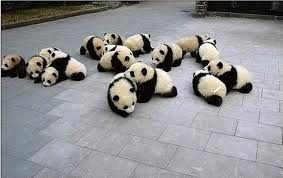
\includegraphics[scale=0.75]{panda.jpg}
\end{center}
\caption{Pande}
\label{fig:pande}
\end{figure}

Na svaku sliku neophodno je referisati se negde u tekstu. Na primer, na slici \ref{fig:pande} prikazane su pande. 
\end{primer}

\begin{primer} I tabele treba da budu u svom okruženju, i na njih je neophodno referisati se u tekstu. Na primer, u tabeli \ref{tab:tabela1} su prikazana različita poravnanja u tabelama.

\begin{table}[h!]
\begin{center}
\caption{Razlčita poravnanja u okviru iste tabele ne treba koristiti jer su nepregledna.}
\begin{tabular}{|c|l|r|} \hline
centralno poravnanje& levo poravnanje& desno poravnanje\\ \hline
a &b&c\\ \hline
d &e&f\\ \hline
\end{tabular}
\label{tab:tabela1}
\end{center}
\end{table}

\end{primer}

\section{K\^{o}d i paket listings}
Za ubacivanje koda koristite paket \textbf{listings}:
\url{https://en.wikibooks.org/wiki/LaTeX/Source_Code_Listings}

\begin{primer}
Primer ubacivanja koda za programski jezik Python dat je kroz listing \ref{simple}. Za neki drugi programski jezik, treba podesiti odgvarajući programski jezik u okviru defnisanja stila.
\end{primer}
\begin{lstlisting}[caption={Primer ubacivanja koda u tekst},frame=single, label=simple]
# This program adds up integers in the command line
import sys
try:
    total = sum(int(arg) for arg in sys.argv[1:])
    print 'sum =', total
except ValueError:
    print 'Please supply integer arguments'
\end{lstlisting}

\begin{lstlisting}[caption={Primer često zadavanog zadatka Fizzbuzz},frame=single, label=simple]
# This program adds up integers in the command line
iex> 
play = fn
  0,0,_ -> "Fizzbuzz"
  0,_,_ -> "Fizz"
  _,0,_ -> "Buzz"
  _,_,c -> "#{c}"
end

IO.puts play.(0,1,2)
play.(0,0,3)
play.(1,0,2)
play.(1,2,15)
\end{lstlisting}


\section{Prvi naslov}
\label{sec:naslov1}


Ovde pišem tekst. 
Ovde pišem tekst. 
Ovde pišem tekst. 
Ovde pišem tekst. 
Ovde pišem tekst. 
Ovde pišem tekst. 
Ovde pišem tekst. 
Ovde pišem tekst. 


\subsection{Prvi podnaslov}
\label{subsec:podnaslov1}

Ovde pišem tekst. 
Ovde pišem tekst. 
Ovde pišem tekst. 
Ovde pišem tekst. 
Ovde pišem tekst. 
Ovde pišem tekst. 
Ovde pišem tekst. 

\subsection{Drugi podnaslov}
\label{subsec:podnaslov2}

Ovde pišem tekst. 
Ovde pišem tekst. 
Ovde pišem tekst. 
Ovde pišem tekst. 
Ovde pišem tekst. 
Ovde pišem tekst. 


\subsection{... podnaslov}
\label{subsec:podnaslovN}

Ovde pišem tekst. 
Ovde pišem tekst. 
Ovde pišem tekst. 
Ovde pišem tekst. 
Ovde pišem tekst. 
Ovde pišem tekst. 

\section{n-ti naslov}
\label{sec:naslovN}

Ovde pišem tekst. 
Ovde pišem tekst. 
Ovde pišem tekst. 
Ovde pišem tekst. 
Ovde pišem tekst. 

\subsection{... podnaslov}
\label{subsec:podnaslovK}

Ovde pišem tekst. 
Ovde pišem tekst. 
Ovde pišem tekst. 
Ovde pišem tekst. 
Ovde pišem tekst. 

\subsection{... podnaslov}
\label{subsec:podnaslovM}

Ovde pišem tekst. 
Ovde pišem tekst. 
Ovde pišem tekst. 
Ovde pišem tekst. 
Ovde pišem tekst. 


\section{Zaključak}
\label{sec:zakljucak}

Ovde pišem zaključak. 
Ovde pišem zaključak. 
Ovde pišem zaključak. 
Ovde pišem zaključak. 
Ovde pišem zaključak. 
Ovde pišem zaključak. 
Ovde pišem zaključak. 
Ovde pišem zaključak. 
Ovde pišem zaključak. 
Ovde pišem zaključak. 
Ovde pišem zaključak. 
Ovde pišem zaključak. 


\addcontentsline{toc}{section}{Literatura}
\appendix
\bibliography{seminarski} 
\bibliographystyle{plain}

\appendix
\section{Dodatak}
Ovde pišem dodatne stvari, ukoliko za time ima potrebe.
HOvde pišem dodatne stvari, ukoliko za time ima potrebe.
Ovde pišem dodatne stvari, ukoliko za time ima potrebe.
Ovde pišem dodatne stvari, ukoliko za time ima potrebe.
Ovde pišem dodatne stvari, ukoliko za time ima potrebe.


\end{document}

